\section{Design}
\label{sec:design}

%\todo{Design goals look rather similar to Pacer.}
The previous section describes an abstract differentially private traffic
shaping strategy.
We now present a traffic-shaping tunnel design that satisfyies DP guarantees.

A traffic shaping tunnel must address three requirements.
%{\bf R1.} It must ensure that the payload is unobservable to an adversary from
%the traffic shape. The packet sizes and timing may be correlated with
%application secrets or the application's sending or receiving rate (\ie flow
%control), which in turn may be secret-dependent.
{\bf R1.} Given a sequence of packets whose sizes and timing reveal the payload,
the tunnel must produce a packet sequence whose sizes and timing do not reveal
information about the payload.
{\bf R2.} It must protect against an adversary observing packets
along the entire path between the tunnel endpoints.
{\bf R3.} It must provide similar levels of reliability, congestion control, and
loss recovery as the original packet sequence.

R1 requires that the tunnel implements DP shaping correctly. Specifically,
it must complete DP decision making and preparation of a shaped buffer within
each interval (as defined in the DP shaping strategy). Moreover, it must be able
to transmit all payload bytes generated from an application within a finite
window length (defined in the DP shaping strategy).
R2 and R3 require that a tunnel implements padding in the outbound packets above
the transport layer so that it is delivered and acknowledged by the destination
and retransmitted upon loss in the same way as application payload.
%R2 requires that a tunnel must ensure that both payload and padding is delivered
%and elicit acknowledgements from the destination and, thus, must apply padding
%in the outbound packets before the transport layer packets are constructed.

\if 0
One way to address all the requirements is to tunnel the transport layer
protocol between the application endpoints through {\sys}'s tunnel.
However, tunneling UDP through any protocol can be inefficient,
and tunneling
TCP through TCP can cause a TCP meltdown \cite{honda2005tcpovertcp,
tcp-meltdown}.
Tunneling TCP through UDP is insecure: TCP between the application end hosts
handles retransmission of lost payload bytes only,
not of any dummy bytes injected between the tunnel endpoints, making padding
observable.
\fi

{\sys} adopts a transport-layer proxy architecture: it transmits
the application byte stream over a transport protocol terminating at the
tunnel endpoints.
This ensures that only one congestion control and reliable delivery mechanism is
active in a tunnel.
In the tunnel, payload and dummy bytes are subject to identical
mechanisms, ensuring that they are indistinguishable to an adversary.
%This architecture satisfies both the security and practical requirements of a
%traffic shaping tunnel.
For ease of implementation, our prototype requires applications to explicitly
connect to a tunnel endpoint.
In principle, {\sys} can also transparently proxy application
connections.

\begin{figure}[t]
    \centering
    %  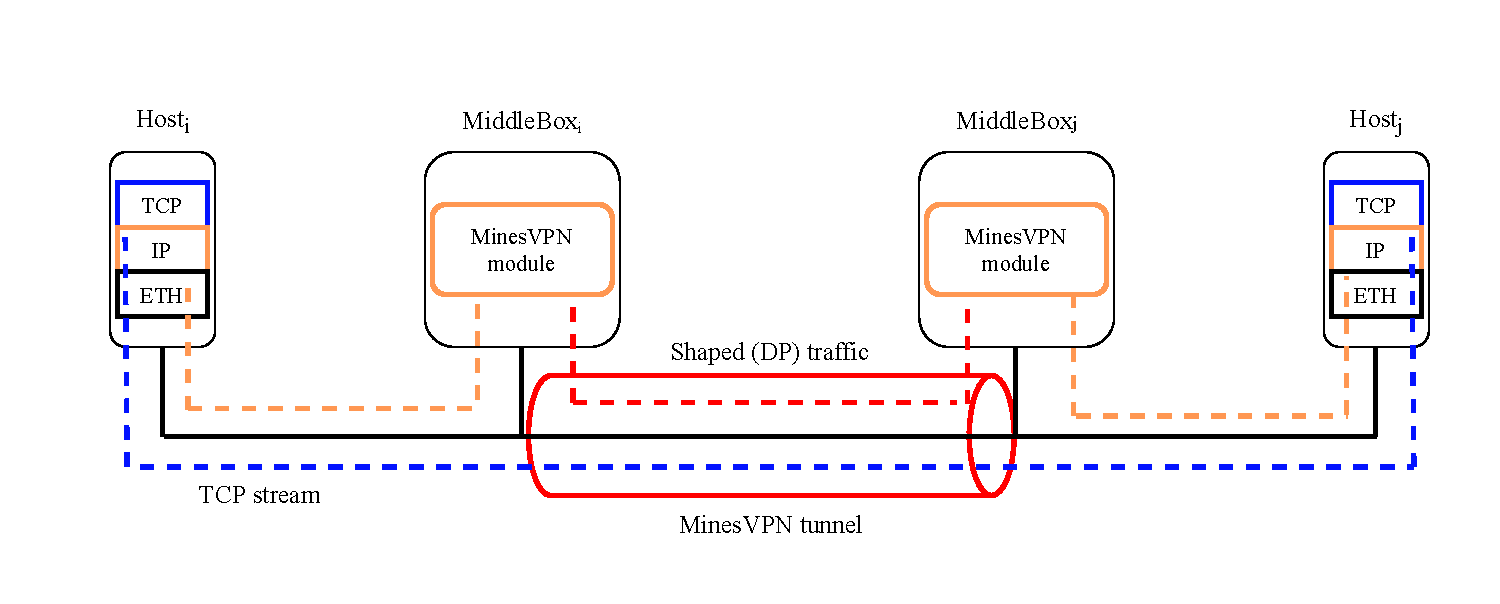
\includegraphics[width=\columnwidth]{figures/Design_highlevel.pdf}
    %  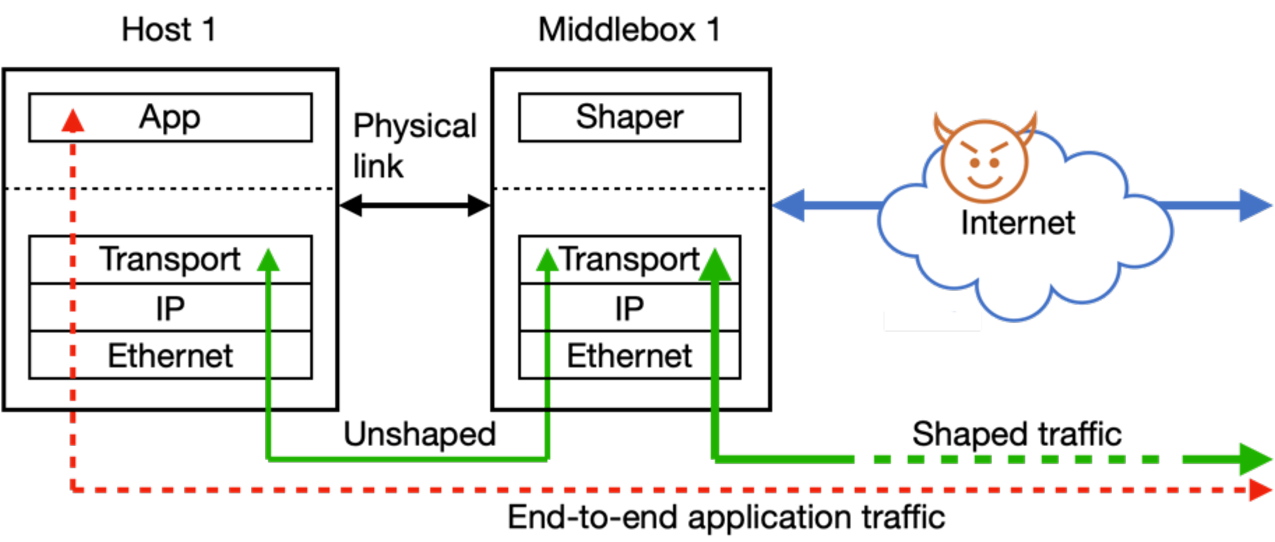
\includegraphics[width=\columnwidth]{figures/minesvpn-overview-half.pdf}
    %  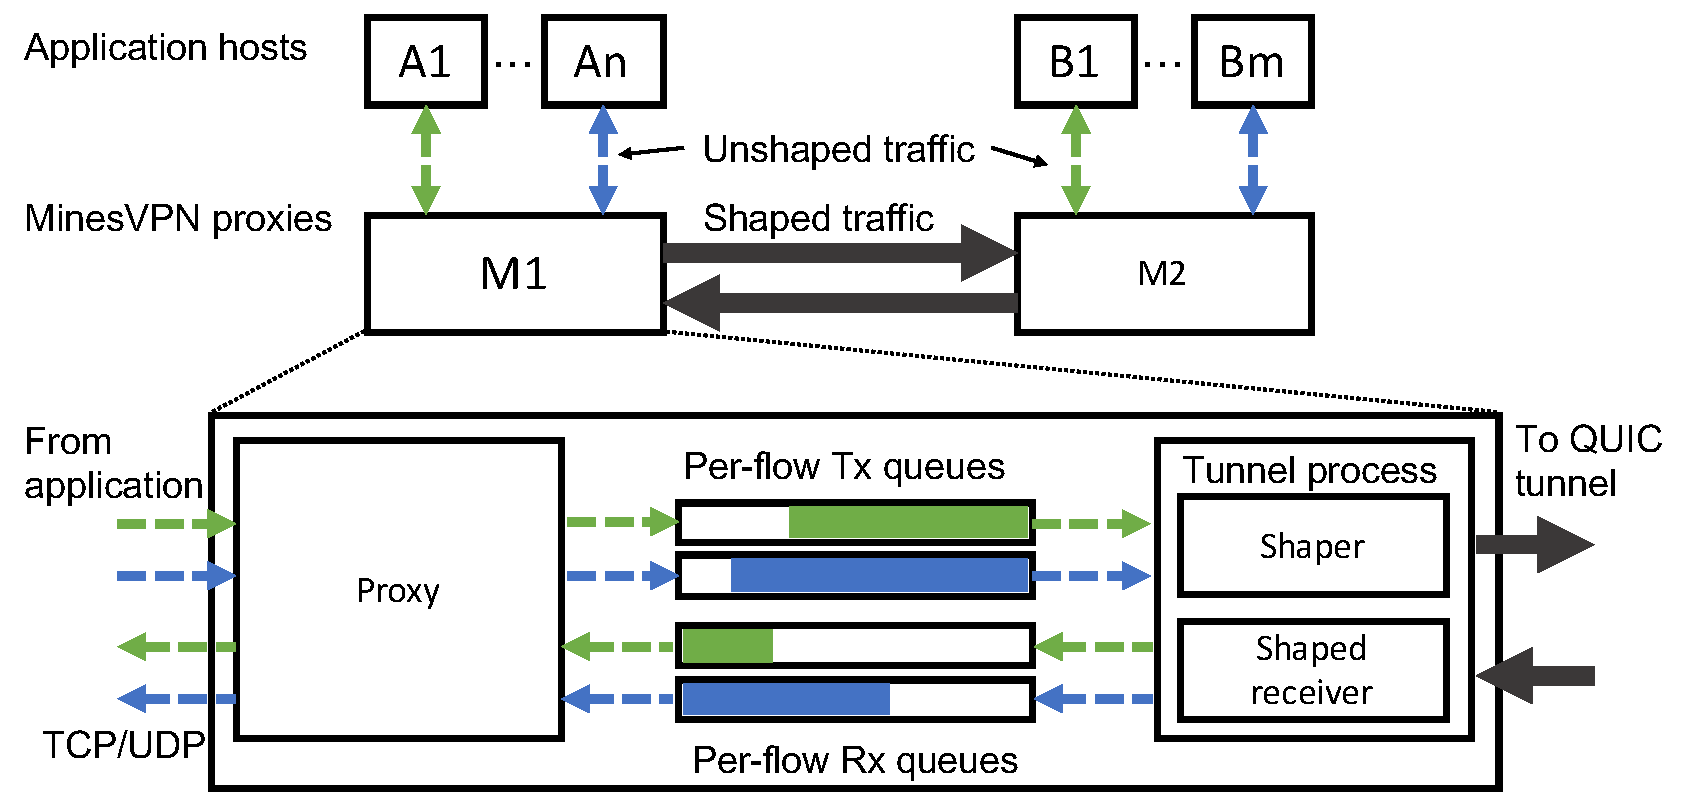
\includegraphics[width=\columnwidth]{figures/minesvpn-arch4.pdf}
    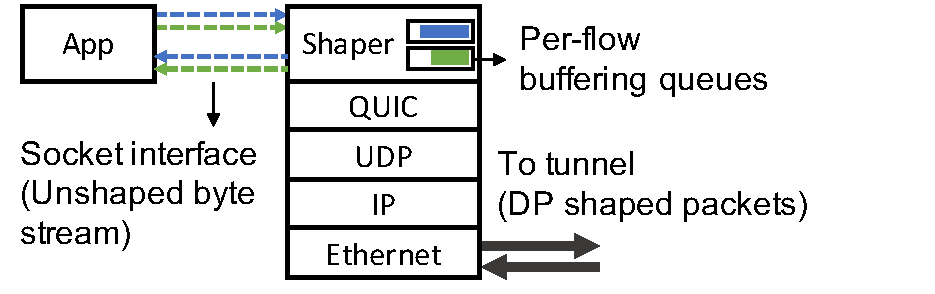
\includegraphics[width=\columnwidth]{figures/design2.pdf}
    \caption{Overview of tunnel design (one endpoint)
        %\am{Update figure}
    }
    \label{fig:minesvpn-overview}
\end{figure}

\subsection{Overview}
\label{subsec:design-overview}

\Cref{fig:minesvpn-overview} shows the design of one endpoint of {\sys}’s
traffic shaping tunnel. A similar endpoint is deployed on the other end of an the tunnel.
%The tunnel endpoints are deployed at both ends of an application’s traffic
%stream.
The endpoints could be integrated with the end hosts or with a gateway at the
edge of an organization’s network. Each tunnel is bidirectional, where the
shape can be configured independently in each direction.

A tunnel endpoint consists of a shaping layer on top of the QUIC protocol,
which in turn runs on top of a standard UDP stack\footnote{In principle, {\sys}
could also rely on a traditional TCP stack.}. The tunnel endpoints establish a
bidirectional QUIC
connection and generate DP-sized transmit buffers in fixed intervals, which
carry payload bytes from one or more application flows.
In the absence of application payload, an endpoint transmits dummy bytes, which are
discarded at the other endpoint.

%An application interacts with the shaping layer through a set of per-flow queues
%carrying the application byte stream. Each flow is mapped to a pair of transmit
%and receive queues.

An application interacts with the shaping layer through a socket connection. For
each application connection, the shaping layer maintains a {\em buffering
queue}, in which it accumulates the application's outbound byte stream before
transforming it into a differentially-private packet sequence.

The security of the tunnel design relies on the key assumption that the traffic
between an application endpoint and the tunnel endpoint is
unobservable to an adversary.
%The security of the tunnel design relies on two key assumptions. First, the
%traffic between an application endpoint and the tunnel endpoint close to it is
%not observable to an adversary, as also mentioned in
%\S\ref{subsec:threat-model}. Secondly, the time required by the shaping layer to
%prepare the DP-sized buffers is independent of application secrets.

\paragraph{Tunnel setup and teardown.}
{When one endpoint of an application initiates communication with
another endpoint, the initiator first establishes a {\sys} tunnel between the
application endpoints before establishing communication with the receiver. The
initiator sends a configuration message to the shaping layer with the source and
destination IP addresses and ports, a reliability flag, and a privacy descriptor.
%\todo{and a tunnel lifetime}.
The reliability flag indicates if the tunnel should provide reliable delivery
semantics or not. The privacy descriptor indicates the DP parameters to be used
for shaping the tunnel traffic.
%\todo{The lifetime indicates the duration for which the tunnel transmits DP
%shaped traffic.}}
%\mis{I don't understand the lifetime: this suggests that someone
%needs to know how long the tunnel needs to exist; doesn't it make more
%sense to have a timeout that says to shut down the tunnel after some
%period of inactivity?}
\mis{About now I keep wanting to say, "No, it's the middlebox" ever time I
see the word endpoint.  I think we need a sentence at the beginning of
Section 4.1 (design overview) that says something like "Although our implementation places tunnel endpoints on a middlebox, for the purposes of our
design, we do not distinguish between the locations of
application endpoints and tunnel endpoints; they could be located on the
same node, or they could be on different nodes as in our implementation.}

Upon receiving a control message, the tunnel endpoint establishes a QUIC
connection with the remote endpoint and configures the reliability semantics
and privacy parameters
%\todo{and tunnel lifetime}
for each direction.
The endpoint also
initializes two QUIC bidirectional streams in the tunnel: control~and
dummy.
The control stream transmits
messages related to the establishment and termination of a connection
between the application endpoints. The dummy stream transmits padding
in QUIC packets in the form of STREAM frames\footnote{We do not use QUIC's
PADDING frames as they do not elicit acknowledgements and hence are
distinguishable from STREAM frames \cite{rfc9000}.}.
%The data streams carry the payload bytes from application flows.

%\todo{After the expiry of the lifetime},
\update{When the tunnel is inactive for a period of time, one of the endpoints
initiates a termination sequence and closes all open QUIC streams and the tunnel
connection.}


\paragraph{Initializing and closing shaped streams.}
%\mis{The sentence that follows desribes setting up a new stream; not
%setting up the tunnel; I think this should be called out separately
%as a step between creating the tunnel and shaping the traffic.}
Once a tunnel is ready, the initiator runs a connection handshake, which is
intercepted in the tunnel.
\todo{The shaping layer establish a new QUIC data stream in
the existing tunnel and maps the new application flow to the new stream.}
The remote tunnel endpoint establishes a connection with the receiver and sets
up the receiver's configurations in the QUIC tunnel.
\todo{When an application flow terminates, the tunnel closes the QUIC data
stream and the connections with the application endpoints.}
The stream setup and closing messages are shaped according to the tunnel's
parameters. \am{Fix the red text.}
%\todo{If a tunnel is already exists between the source and destination IP
%addresses with the same configurations, the shaping layer maps the new
%application flow with one of the unused data streams in the existing tunnel.}
%{\todo{After the expiry of the lifetime}, one of the tunnel endpoints initiates
%a termination sequence and closes all open QUIC streams and the tunnel
%connection.}


\paragraph{Traffic shaping within a tunnel.}
The shaping layer in a tunnel endpoint converts the byte stream of one or more
application flows into a sequence of network packets whose sizes and timing
follow a distribution that guarantees DP.
At periodic intervals, \update{it performs a DP measurement to determine the
number of bytes $\qlendp$ to be~transmitted according to the tunnel's DP
parameters}. It prepares a buffer consisting of $\payload$ payload bytes
and $\dummy$ dummy bytes, where $\payload$ is the minimum of $\qlendp$ and the
application bytes available in the buffering queue, and $\dummy = \qlendp -
\payload$, which may lie between 0 and $\qlendp$. The shaping layer then passes
the buffer along with the position and length of the padding to the QUIC~layer.

QUIC transforms the buffer into one or more STREAM frames based on the
congestion window, the flow window of the receiver endpoint, and the MTU
(maximum transmission unit). It
places the padding bytes into a dummy STREAM frame. QUIC packages the frames
into packets, whose length is at most MTU
minus the length of the headers and whose payload is
encrypted. QUIC forwards the packets to the UDP layer, which subsequently
transmits the prepared packets as quickly as it can, given the line rate of the
NIC.

{\sys} configures the periodic interval such that the shaping layer can prepare
each DP buffer within an interval. If the preparation time for a buffer exceeds
the interval, the shaping layer discards the buffer. This ensures that the
buffering queue length does not grow significantly, which in turn controls the
overhead incurred due to DP shaping.
%\am{Note this is secure only if delays due to cc. All other delays should be
%properly masked.}
%
%We elaborate on the DP model in \S\ref{sec:dp}.
We analyze the impact of the buffering queue~length and the periodic interval
length on privacy guarantees, bandwidth overheads, and latency overheads in
\S\ref{sec:eval}.

\paragraph{Inbound traffic processing within a tunnel.}
A tunnel endpoint receives shaped packets from the tunnel and applies inverse
processing on each packet.
QUIC receives the packet and
sends an ACK to the sender. Subsequently, it decrypts the packet, discards the
dummy frame, extracts the payload bytes from the remaining STREAM frames, and
forwards the payload bytes to the application.

%\paragraph{Configuring privacy requirements.}
%\todo{By default, each flow sent through a single tunnel is subject to the same
%DP parameters. Furthermore, the tunnel aggregates the payload from concurrent
%flows to amortize the padding overheads of DP. However, an application can
%choose to configure the DP parameters separately for each of its flows. Each
%flow with distinct DP parameters requires a separate tunnel.}


%%%\Cref{fig:minesvpn-overview} gives an overview of {\sys}'s design.
%%%Tunnel endpoints (\eg M1 and M2) integrate
%%%shaping within the QUIC protocol, which runs on top of a standard UDP stack.
%%%The
%%%QUIC stack is used by M1 and M2 to communicate with each other and with other
%%%tunnel endpoints, as well as with their local application endpoints A1,
%%%..., An and B1, ..., Bm (respectively)\footnote{In principle, {\sys} could
%%%also
%%%rely on a traditional TCP or a UDP stack based on applications' reliability
%%%requirements.}.
%%%For two application endpoints to communicate, say A1 and B1, a bidirectional
%%%connection is set up between M1 and M2, through which the application traffic
%%%is
%%%shaped and transmitted.
%%%Specifically, M1 terminates the transport connection of A1, and transforms the
%%%byte stream of A1 to B1 into a shaped traffic stream, which is then
%%%transmitted
%%%to M2. Similarly, M2 terminates the transport connection of B1 and shapes the
%%%byte stream from B1 to A1. M1 and M2 shape the traffic in each direction
%%%independently.
%%%
%%%\paragraph{Traffic shaping within a tunnel.}
%%%\todo{A tunnel endpoint converts an application's byte stream into a sequence
%%%of
%%%network packets whose sizes and timing follow a differentially private
%%%distribution.}
%%%%\am{Goes back to my question, can we prove that periodic timing + DP burst
%%%%sizes within periodic intervals $\Rightarrow$ overall DP shape?}
%%%For this, a tunnel endpoint relies on the \todo{primitive} of a {\em buffering
%%%queue}, in which it accumulates the application byte stream before
%%%transforming
%%%it into a differentially-private packet sequence.
%%%
%%%For example, when the tunnel endpoint M1 receives an unshaped byte stream from
%%%its local end host A1, which is destined for end host B1, M1 enqueues the byte
%%%stream into the buffering queue. After every periodic time interval $T$, M1
%%%computes the number of bytes $n$ to be transmitted in the next interval
%%%according to the DP parameters of the corresponding tunnel between M1 and M2.
%%%M1
%%%prepares a buffer with a number of bytes $r$ that is the minimum of the number
%%%of the number of application bytes available in the buffering queue and $n$,
%%%and
%%%generates additional $d = n - r$ dummy bytes if required. M1 then adds a
%%%padding
%%%header to the buffer to indicate the position and length of the padding,
%%%and encrypts the buffer and the padding header. Finally, M1 transforms the
%%%buffer into one or more network packets of at most MTU length (maximum
%%%transmission unit) and transmits the prepared packets as fast as it
%%%can given the line rate of the connected NIC and the congestion conditions of
%%%the downstream network.
%%%
%%%The size of the buffering queue and the length of the periodic intervals
%%%determine the tradeoffs between privacy guarantees, bandwidth overheads, and
%%%latency overheads of {\sys}. We elaborate on the DP model in \S\ref{sec:dp}
%%%and
%%%evaluate the tradeoffs in \S\ref{sec:eval}.
%%%\am{explicitly mention dropping of queue data if not consumed within fixed
%%%interval.}
%%%
%%%\if 0
%%%When a tunnel endpoint M1 receives an unshaped byte stream from its local end
%%%host A1, which is destined for end host B1, M1 transforms the byte stream
%%%into
%%%a
%%%sequence of buffers whose sizes follow a noise distribution defined by the DP
%%%parameters of the corresponding tunnel between M1 and M2, and which are then
%%%transmitted at periodic intervals.
%%%Specifically, after every periodic time interval $T$, M1 computes the number
%%%of
%%%bytes $n$ to be transmitted in the next interval according to DP. M1 prepares
%%%a
%%%buffer with a number of bytes $r$ that is the minimum of the number of bytes
%%%available in the application's byte stream and $n$ and generates additional
%%%$d$
%%%= $n - r$ dummy bytes if required. M1 then adds a padding header to the
%%%buffer
%%%to
%%%indicate the position and length of the padding, encrypts the buffer and the
%%%padding header, adds the protocol headers of the tunnel's network stack, and
%%%transmits the prepared packets as fast as it can given the line rate of the
%%%connected NIC and the congestion conditions on the downstream network.
%%%\fi
%%%
%%%
%%%\paragraph{Inbound traffic processing within a tunnel.}
%%%Each tunnel endpoint receives shaped packets from the tunnel and process them
%%%in
%%%the reverse order. For instance, when the tunnel endpoint M1 receives packets
%%%from M2, which are sent from end host B1 to A1, M1 strips the tunnel protocol
%%%headers, decrypts the buffer, discards the dummy bytes, and forwards the
%%%payload
%%%bytes to A1.

%%The packets are
%%processed in the endpoint in the reverse order: the tunnel protocol headers are
%%stripped, the content is decrypted and payload bytes are forwarded to the end
%%host, while dummy bytes are discarded at the endpoint.

\if 0
\subsection{Security Guarantees \am{to be revised}}
\label{susbec:design-security}
%{\sys}'s design satisfies the security requirements as follows.

\am{We should show design follows the DP spec and implementation follows the
design. Therefore, we have a secure solution by design and construction.}
\am{Combine security analysis of design and implementation and move to
evaluation?}
{\sys}’s design provides the following security property: an adversary cannot
infer application secrets \todo{or the number of active participants} by
observing the tunnel traffic. This property holds because:
%
%{\bf S1.} The traffic between an application endpoint and the tunnel endpoint
%close to it is not observable to an adversary (by assumption).
%
{\bf S1.} All payload traffic of a sensitive flow passes through a tunnel and is
subjected to shaping and encryption.
%
{\bf S2.} The shaping layer prepares differentially-private sized buffers and
passes the buffers to QUIC in fixed intervals. Subsequently, the QUIC layer may
transmit the buffers in one or more packets. However, by the post processing
argument of DP \citeme{dp-postprocessing}, the shape of the packets still
provides DP. (The proof of DP is in \todo{\S\ref{appendix:dp}}.)
%
%\todo{{\bf S2.} The tunnel continuously transmits DP shaped traffic, which
%hides the start and end times of application transmissions.}
%
\todo{{\bf S3.} The privacy guarantees of a tunnel are configured before the
start of application transmission and do not change during the tunnel lifetime.}
\todo{{\bf S4.} The time required by the shaping layer to
prepare the DP-sized buffers is independent of application secrets. This is
because {\sys}'s periodic interval is configured such that it can handle all DP
sizes. Thus, any delays in transmitting the buffers can only arise due to
congestion or packet losses in the tunnel network, which are secret-independent
events.}
\fi

%\todo{Note: If we want this to be completely transparent, we might have to do
%some IP Spoofing and will have to include that in our mechanism}

%\subsection{Shaping Module}
%This module has the following responsibilities as a sender:
%\begin{itemize}
%    \item Determine the number of bytes (n) to send in the next time slot
%    \item Obtain 'n' bytes from the Non-DP Queue
%    \item Add dummy bytes if necessary (if Non-DP Queue size < n)
%    \item Add the DP Header populated with all the necessary information
%    \item Encrypt the payload (n bytes of data + DP header)
%    \item Send it out to the other middle-box
%\end{itemize}
%
%It also acts as a receiver and performs the following tasks:
%\begin{itemize}
%    \item Decrypt the payload
%    \item Obtain the DP header to determine padding, actual destination etc
%    \item Extract the actual payload and send it to the Middle-box Module
%\end{itemize}

%\begin{table}[t]
%    \centering
%    \renewcommand{\arraystretch}{1.2}
%    \begin{tabular}{lll}
    %        \toprule
    %        {\bf Outer/Inner} & {\bf TCP} & {\bf UDP}
    %        \\
    %        \midrule
    %        {\bf TCP} & meltdown & inefficient
    %        \\
    %        {\bf UDP} & insecure & inefficient
    %        \\
    %        \bottomrule
    %    \end{tabular}
%    \caption{Impact of tunneling a transport inside transport}
%    \label{tab:transport-in-transport}
%\end{table}


